\subsection{标量环的扩张}

设 A, A' 为两个交换环， \(\rho:A\to A'\) 为环同态，M 为 A-模，M' 为 A'-模，且 \(f:M\to M'\) 为从 M 到 M' 的 A-同态（相对于 \(\rho\) ）。复合映射 \(M\xrightarrow{f}M'\xrightarrow{\phi_{M'}^{\prime\prime}}\bigwedge_{A'(M')}\) 是从 M 到 A-代数 \(\bigwedge_{A'(M')}\) 的 A-线性映射，并且，由于 \(f(\mathbf{M}) \subset \mathbf{M}'\) 的元素在 \(\bigwedge_{\mathbf{A}'}(\mathbf{M}')\) 中平方为零，存在（第 1 号，命题 1）一个且仅一个代数的 A-同态 \(f'': \bigwedge_{\mathbf{A}}(\mathbf{M}) \to \bigwedge_{\mathbf{A}'}(\mathbf{M}')\) 使图表交换

\begin{enumerate}
\def\labelenumi{(\arabic{enumi})}
\setcounter{enumi}{11}
\tightlist
\item
\end{enumerate}

\pandocbounded{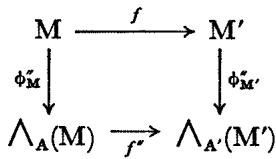
\includegraphics[keepaspectratio]{images/part003_899f4c21.jpg}}

和 \(f''\) 是分次代数同态。立即可以推出，如果 \(\sigma: A' \to A''\) 是另一个环同态， \(M''\) 一个 \(A''\) -模， \(g: M' \to M''\) 一个 \(A'\) -同态（相对于 \(\sigma\) ) 且 \(g'': \bigwedge_{A'}(M') \to \bigwedge_{A''}(M'')\) 相应的 \(A''\) -代数的同态，则复合的代数 A-同态

\[
\bigwedge_ {\mathbf {A}} (\mathbf {M}) \xrightarrow {f ^ {\prime \prime}} \bigwedge_ {\mathbf {A} ^ {\prime}} (\mathbf {M} ^ {\prime}) \xrightarrow {g ^ {\prime \prime}} \bigwedge_ {\mathbf {A} ^ {\prime \prime}} (\mathbf {M} ^ {\prime \prime})\tag{13}
\]

对应于复合 A-同态 \(g \circ f: \mathbf{M} \to \mathbf{M}''\) （相对于 \(\sigma \circ \rho\) ）。

命题 8. 设 A、B 为两个交换环， \(\rho: A \to B\) 一个环同态，且 M 是一个 A-模。典范扩张

\[
\psi : \bigwedge_ {\mathbf {B}} (\mathbf {B} \otimes_ {\mathbf {A}} \mathbf {M}) \rightarrow \mathbf {B} \otimes_ {\mathbf {A}} \bigwedge_ {\mathbf {A}} (\mathbf {M})
\]

的典范扩张是一个分次 B-代数同构，这里所指的 B-线性映射是 \(l_{B} \otimes \phi_{M}^{\prime\prime}: B \otimes_{A} M \to B \otimes_{A} \bigwedge_{A}(M)\) 。

证明源自 §5 第 4 号命题 5 的证明，只需将 T 换为 \(\bigwedge\) ，并将 \(\phi_{\mathbf{M}}\) 换为 \(\phi_{\mathbf{M}}^{\prime \prime}\) 。

